\section{Theorie}
\label{sec:Theorie}
Ein Laser (Light Amplification by
Stimulated Emission of Radiation)
besteht aus einem Resonator,
einer Pumpquelle und einem aktivem Lasermedium.
Damit ist es möglich, monochromatisches Licht mit einer
hohen Inensität und Kohärenz zu erzeugen.

\subsection{Absorption und Emission}
\label{subsec:absorption_und_emission}
Um die Funktionsweise eines Lasers
zu verstehen, ist es notwendig zunächst
die Wechselwirkung eines Niveau System
mit einem Strahlungsfeld $\rho(\nu)$ zu betrachten
Dazu zählen zum einen die Absorption eines Photon
und sowohl induzierte als auch spontane Emission eines Photon.
Zunachst soll der Fall
eines 2-Niveau Systems betrachtet
werden, wobei zwischen der Besetzungszahl $n_1$
der Atome im Grundzustand
und der Besetzungsdicht $n_2$
der Atome in angeregten
Zustand unterschieden wird.
Besitzt nun Beispielsweise ein
Photon die Energie des Übergangs
kann es von einem Atom im Grundzustand
absorbiert werden und das Atom geht in den
angeregten Zustand über. Atome im angeregten
Zustand können über spontane Emission
wieder in den Grundzustand zurückkehren
indem sie ein Photon mit der Energie
des Übergangs emittieren.
Dieser Übergang lässt ebenfalls
mit ein einfallendes
Photon hervorrufen.
Das so emittierte Photon besitzt gleiche
Energie, Phase und Ausbreitungsrichtung
wie das einfallende Photon,
üblicherweise ist dabei die Rede von
induzierte Emission.
Die Abbildung \ref{fig:ab_em} enthält die drei
zuvor beschriebenen möglichen Wechselwirkung.
\begin{figure}
  \centering
  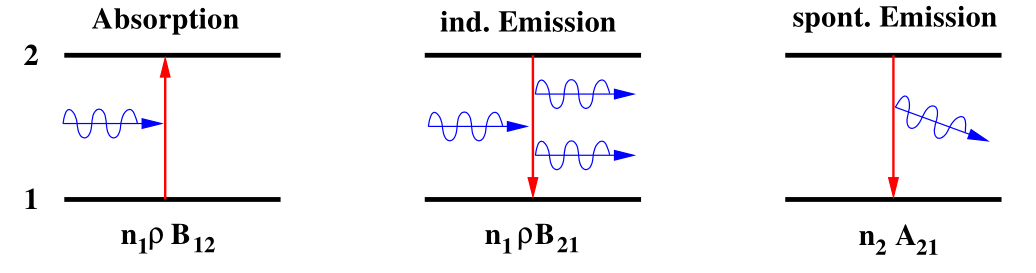
\includegraphics[width=0.7\textwidth]{figures/ab_und_emiss.PNG}
  \caption{Schematische Darstellung
  für die möglichen Wechselwirkung
   eines Strahlungsfeld
  mit einem 2-Niveau System. \cite{sample}}
  \label{fig:ab_em}
\end{figure}

Die Anzahl der so
pro Volumeneinheit und pro Sekunde
absorbiert/emittierten Photonen $\dot{N}$,
ergeben sich mit den Einsteinkoeffizienten $A_21$, $B_21$ und $B_12$
und der Energiedichte $\rho$ des Strahlungsfeldes zu
\begin{align}
& \text{Absorption}   &\dot{N}_A   &= n_1 \rho(\nu)B_{12},\\
& \text{induzierte Emission}   &\dot{N}_{IE}&= n_2 \rho(\nu)B_{21},\\
& \text{spontane Emission}   &\dot{N}_E   &= n_2 \rho(\nu) A_{21}.
\end{align}

Die Einsteinkoeffizienten $A_21$, $B_21$ und $B_12$
geben ein Maß für die Übergangswahrscheinlichkeiten an.
Für eine verlustfreie Vorgang
$(n_1+n_2=const.)$ ändern sich die Bestzungszahlen
gleichermaßen und es ergeben sich folgende
Ratengleichungen für die Besetzungszahlen
\begin{align}
\frac{\symup{d} n_1}{\symup{d} t} &=-n_1 B_{21}\rho + N_2 B_{21} \rho + n_2 A_{21}\\
\frac{\symup{d} n_2}{\symup{d} t} &=+N_1 B_{12}\rho - n_2 B_{21} \rho - n_2 A_{21}.
\end{align}
Damit eine dauerhafte Verstärkung
und Kohärenz des Strahlungsfeld gegeben ist,
muss mehr induzierte als spontane Emission
statt finden. Um dies zu
erreichen wird eine Besetzungsinversion
zwischen Angeregtem- und Grundzustand
erzeugt.
Da im thermischen Gleichgewicht
die Besetzungszahlen sich nach der
Maxwell-Boltzmann-Verteilung
richtet, ist der Grundzustand höher
besetzt als der angeregte Zustand.
Um eine Besetzungsinversion zu erreichen
muss somit dem System kontinuierlich
Enerige Beispielsweise durch
Elekronenstöße oder
optische Anregung zugeführt werden.
Dieser Vorgang wird auch Pumpen genannt.



\subsection{Konzeptioneller Aufbau des allgemeinen Lasers,
sowie des Helium-Neon-Lasers}
\label{subsec:konzeptioneller_aufbau}

Wie schon in Abschnitt \ref{subsec:absorption_und_emission}
beschrieben, besteht ein Laser konzeptionell aus Lasermedium,
Pumpquelle und Resonator.\\
In Abbildung \ref{fig:laserkonzept} ist gezeigt,
wie ein Laser prinzipiell aufgebaut ist.
In Abschnitt \ref{subsec:absorption_und_emission}
wurde bereits auf das grundsätzliche Zusammenspiel von Lasermedium
und Pumpquelle eingegangen.\\
Aufgabe des Resonators ist es nun dafür zu sorgen,
die Strecke, die der Laserstrahl innerhalb
des Lasermediums durchläuft, zu maximieren. Dies ist notwendig,
damit dem Laserfeld möglichst viel Energie zugeführt
werden kann. Um dies zu gewährleisten besteht der Resonator
aus einem totalreflektierenden und einem teilreflektierenden Spiegel,
deren Spiegelflächen von der optischen Achse durchtoßen werden.
(Siehe Abbildung \ref{fig:laserkonzept})
Auf der Seite des teilreflektierenden Spiegels wird der Laserstrahl
zur Verwendung ausgekoppelt.\\
Für die Bauart der Spiegel kann separat die Wahl zwischen planparallel und
sphärisch getroffen werden. Allerdings muss gewährleistet werden, dass
nur sehr geringe Verluste auftreten. Daher wird
der Aufbau üblicherweise so gewählt, dass die Brennpunkte der beiden Spiegel
identisch sind.
Um sicherzustellen, dass die Energiezufuhr des Laserfelds größer ist als
die Verluste, muss gelten
\begin{align}
  0 \leq g_{1} \, g_{2} \less 1 \, .
\end{align}
Dabei bezeichnen $g_{i}$ die Resonatorparameter.
Diese ergeben sich durch
\begin{align}
  g_{i} = 1 - \frac{L}{r_{i}} \, ,
\end{align}
aus Resonatorlänge $L$ und den Krummüngsradien der Spiegel $r_{i}$.

\FloatBarrier
\begin{figure}
  \centering
  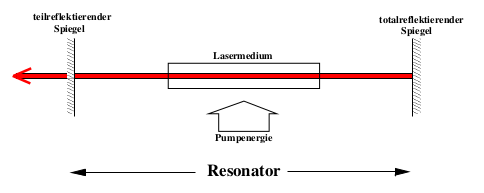
\includegraphics[width=0.75\textwidth]{figures/laserkonzept.png}
  \caption{Prinzipieller Aufbau eines Lasers.\cite{sample}}
  \label{fig:laserkonzept}
\end{figure}
\FloatBarrier

In dem in diesem Protokoll beschriebenen
Versuch wird ein Helium-Neon-Laser verwendet.
Bei diesem wird ein Gasgemisch aus Helium und
Neon (Verhältnis $5:1$, Druck $\sim \SI{133}{\pascal}$) verwendet.
Dabei dient Neon als Lasermedium und Helium wird für das Pumpen
des Lasers eingesetzt. Um die Besetzungsinversion im Lasermedium
zu erreichen, werden zunächst die Heliumatome über ein
eletrisches Feld in kurzzeitig stabile Zustände gebracht.
Diese können nun ihre
überschüssige Energie über Stöße an die Neonatome abgegeben,
wodurch die notwendige Besetzungsinversion erreicht wird.
Der Helium-Neon-Laser weist ein diskretes Spektrum auf, dessen
prominenteste Linie bei $\lambda = \SI{632.8}{\nano\meter}$ im
roten Bereich des sichtbaren elektromagnetischen Spektrums liegt.






\subsection{Lasermoden}
\label{subsec:lasermoden}
Bei einem Laser ist die
Resonatorlägne $L$ ist deutlich größer
als die Wellenlängen $\lambda$. Deshalb erfüllen viel Frequenzen
die Resonanzbedingung für eine stehende Welle im Resonator.
Die longitudianle Mode $q$ entspricht der Anzahl der Wellenlängen
im Resonator. Zusätzich bilden sich im Resonator
Aufgrund von Verkippung oder Spiegelunebenheiten
transversale Moden aus.
Eine gesamte Mode des Resontors wird
$\text{TEM}_{lpq}$ (transverse electromagnetic mode)
gennant. Dabei entsprechen $l$ und $p$ die Knoten in
x- und y-Richtung und werde auch
transversale Modenzahl gennant.
Die beobachtbare Intensitätsverteilungen für bestimme Moden
ergeben sich aus der Feldverteilung $E_{lpq}$, die
sich mit Hilfe von Laguerre-Polynome $L_p^q(u)$
berechnen lassen. Für
die Intensitätsverteilungen der $\text{TEM}_{00}$ Grundmode folgt Beispielsweise
eine Gausverteilung der Form
\begin{align}
I(d)=I_0\exp\left(-2\left(\frac{d-d_0}{\omega}\right)^2\right). \label{eqn:TEM00}
\end{align}
mit der Maximalintensität $I_0$, dem Abstand zur optischen Achse $(d-d_0)$
und dem Strahldurchmesser $2\omega$.
